\chapter{Geometric Modelling, Gridding and Visualization}
\textit{by Bj\"orn Zehner}

\bigskip

Geometric modelling and 3D visualization are two aspects that are important for simulation. The first one is a preprocessing step in which a 3D description of the input model is set up which is later needed for generating the 3D grid on which the simulation is run and for setting the different parameters on the grid's cells and the initial and boundary conditions. The latter one  is needed because the output of the simulation is usually a vast amount of numbers. Visualization (and Virtual Reality) deals with the the question of how to represent these numbers in an intuitive and comprehensible way. Examples of this are the visualization of tensor fields from geomechanics \cite{zehner:2006} or of scalar fields with uncertainty \cite{Zehner:2010:Uncertainty}.

\begin{figure}[tb]
\begin{center}
\includegraphics[width=0.99\linewidth]{figures/geomod_and_vis_fig_1}
\caption{Processing workflow from geological interpretation and geometrical modelling via simulation to visualization.}
\label{geomod_and_vis:1}
\end{center}
\end{figure}

Figure \ref{geomod_and_vis:1} shows the overall processing workflow from data interpretation via modelling and simulation to visualization, as it is used in the geoscience domain. As a first step, a 3D model that describes the subsurface is constructed from the field data provided. While this 3D model construction can be done using CAD software for geotechnical and engineering applications, the more complicated and irregular geological structures require specialized software. One program that is commonly used by many universities, state agencies, oil companies and alike for this task is GOCAD\footnote{GOCAD: \texttt{http://www.pdgm.com}} from Paradigm Ltd, another one is Petrel\footnote{Petrel: \texttt{http://www.slb.com}} from Schlumberger. The next necessary step is the generation of 3D simulation grids from the geometrical models. For reservoir simulation purposes, the use of hexahedral grids and finite difference simulation methods is more common and the construction of these grids works quite well in most modelling packages. However, to represent complicated 3D geological structures, such as fault systems, unstructured grids that use tetrahedra are more suitable. In order to generate these grids, the modelling software has to be used to construct a boundary representation of the 3D model from which the simulation grid can be generated using e.g. TetGen\footnote{TetGen: \texttt{http://tetgen.berlios.de/}}, a software that is open source for research purposes. TetGen also recognizes if the volume is partitioned into subspaces and assigns corresponding identifiers to the generated tetrahedra. Further the geometries from the 3D Model can be used to set the initial and boundary conditions, for example a predefined flow on all vertices along a line.

After running the simulation the results need to be visualized. A very comprehensive C++ library that provides most of the standard algorithms for visualizing scientific data is the Visualization Toolkit (VTK)\footnote{VTK: \texttt{http://www.vtk.org}} \cite{Schroeder1996}. VTK is pipeline-oriented and provides different filters that each take an input data set, do some processing (such as isosurface extraction) and forward the result to the next filter or an object that visualizes it. In this way complicated pipelines can be constructed in order to assess the data. VTK also defines its own file formats and the finite element software OpenGeoSys (OGS) can output simulation results directly in this format. The VTK library can be used to implement a full visualization application. This has been done, for example, with the OGS Data Explorer (see chapter on data processing). Further the open source software Paraview\footnote{Paraview: \texttt{http://www.paraview.org}} is based on VTK and makes most of the filters available within a graphical user interface.

If synoptic views are created that visualize the simulation results together with the geometrical model and with other data on which this model is based, the display quickly becomes cluttered and it becomes difficult for the viewers to grasp the spatial interrelationships of the data. Further simulation results are often discussed in small groups or are presented to stakeholders who are not familiar with the interpretation of the visualization shown to them, and for this reason have problems understanding it. Stereoscopic visualization on high resolution display walls can help to overcome these problems, as they provide a real 3D impression that is easier for the viewers to understand and can show much more detail. However, these display walls are usually more complicated to use as they involve several projectors that are run by a computer cluster and so require specialized software. The display at the UFZ-Helmholtz Centre for Environmental Research\footnote{Homepage of UFZ's Visualization Center:\texttt{http://www.ufz.de/index.php?en=14171}},
for example, uses 13 SXGA+ projectors in a theater-like configuration with a large rear screen, two side screens and a projection on the floor. It can be used either as an immersive VR display or as a display where the rear screen and the floor are used in VR mode, while the side screens show additional 2D information, such as maps, in order to help the users orient themselves in large-scale regional models or borehole data and logs (see Figure \ref{geomod_and_vis:2}). A full description of the system, its design concept and the use as visual information system can be found in \cite{Zehner2010:2D3D}.

\begin{figure}[tb]
\begin{center}
\includegraphics[width=0.99\linewidth]{figures/geomod_and_vis_fig_2}
\caption{Combined 2D and 3D visualization in the UFZ's visualization center as suggested in \cite{Zehner2010:2D3D}. The rear screen and the floor are used to show the 3D model using head-tracked stereoscopic visualization. On the side screens additional information is shown, such as the stratigraphic profile of a borehole, graphs or a map on which the position of the user is indicated and the direction in which he or she is looking. 2D- and 3D-Views are coupled.}
\label{geomod_and_vis:2}
\end{center}
\end{figure}

To run these kind of systems the open-source scenegraph OpenSG\footnote{OpenSG: \texttt{http://www.opensg.org/}} \cite{Reiners2002} can be used very well as it supports the distribution of the scenegraph. A visualization application runs on the master computer, assembles the scene and reacts on the user input. The scenegraph itself and the changes to it are always distributed to the remote computers on which OpenGL is used to render the scene. The scenegraph is relatively well documented and comes with examples that show different features, for example how to run a display wall with a computer cluster. The UFZ uses a commercial application, VRED from PI-VR GmbH\footnote{VRED: \texttt{www.pi-vr.de}} that is based on OpenSG to run its visualization center. We have extended VRED using OpenSG and Nokia's Qt Toolkit for the graphical user interface. We also have extended VTK with a vtkOpenSGActor class so that content that has been created using a VTK pipeline can be easily converted on the fly into OpenSG format. In this way we have integrated some standard features, such as isosurface extraction from scalar fields or glyph rendering and streamline computation for vector fields, into VRED.

As we have seen, the whole workflow and data processing involves several software packages and libraries that are each specialized for a certain step of the workflow. For this reason the data have to be converted between these different formats and the information is distributed across several files that must be viewed with several software packages. We have experimented with using GOCAD as a tool for geometric modelling, data exchange with our project partners and model maintenance. GOCAD provides import and export functionality to different data formats, such as ArcGIS Shape files, and it can be extended, using C++ and a plugin mechanism, so that we can add our own algorithms, exporters and importers. In contrast to the often applied way to write data converters that read data in GOCAD ASCII format and output the desired file type, our chosen way of extending GOCAD has the advantage that we can make use of the topological information that GOCAD keeps track of internally but does not write to the files. Further we have access to the data that describe the appearance of the different objects in GOCAD (e.g. line width or colour of a surface), so that we can very easily create the same visualization using other formats. In order to provide an easier and more rapid data exchange we have added some modelling functionality and the necessary interfaces between GOCAD and Gmsh, TetGen, VTK, OpenSG and our finite element simulation software OpenGeoSys. In this way we support the processing of the data as is described in Figure \ref{geomod_and_vis:3}. 

\begin{figure}[tb]
\begin{center}
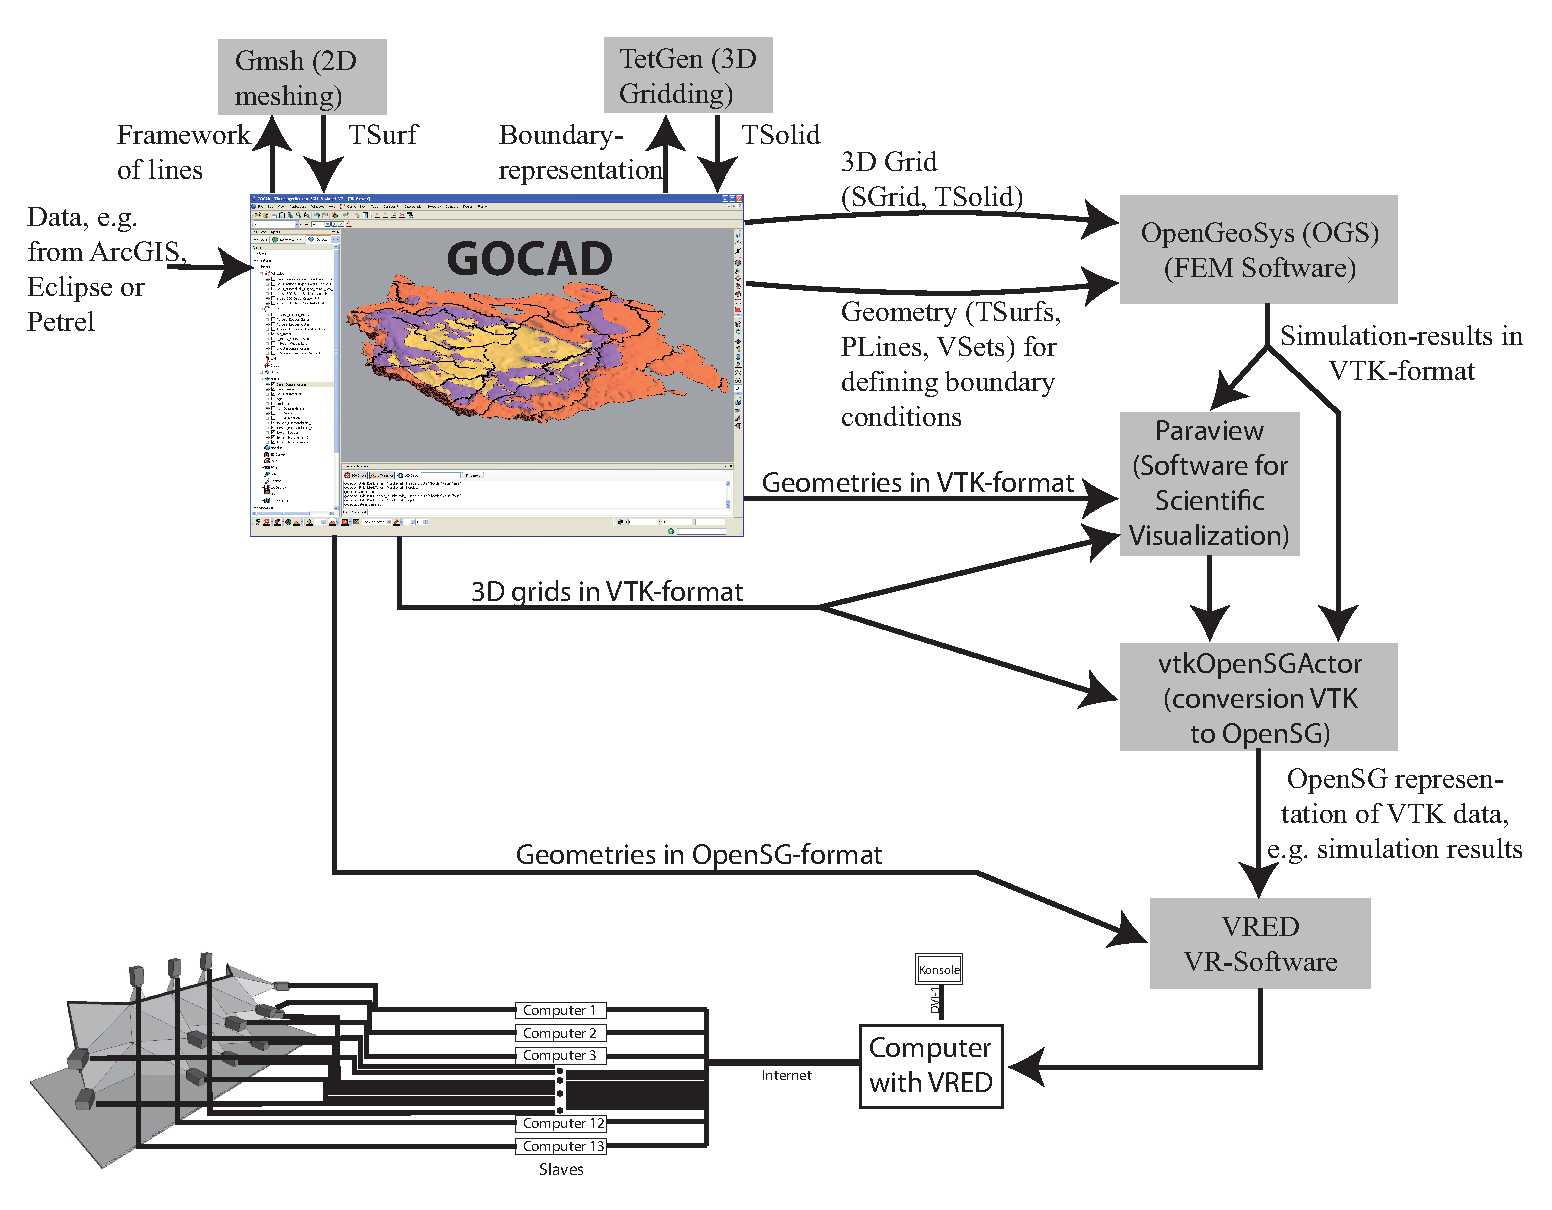
\includegraphics[width=0.99\linewidth]{figures/geomod_and_vis_fig_3}
\caption{Processing pipeline for the data from geometrical modelling through simulation to visualization.}
\label{geomod_and_vis:3}
\end{center}
\end{figure}

In order to generate the simulation grids, GOCAD already provides algorithms that generate a structured (hexahedral) grid which can be fitted to the geology that delineates the actual reservoir. However, as mentioned earlier, with regard to complicated reservoirs a (tetrahedral) mesh would be preferable. For many geometrical models, one critical step is the conversion from the surface- or boundary-based 3D model to the 3D grid, because this step requires the surface model to fulfil different constraints. In order to generate tetrahedral grids, the quality of the triangular meshes must be higher than is normally required for illustration, communication and discussion purposes. The mesh should consist of triangles with not too large an aspect ratio (longest side length divided by shortest side length). The lines, where one surface intersects another one or is connected to it, for example at the contact of a stratigraphic layer and a fault, are also critical. As is shown in Figure \ref{geomod_and_vis:4}, it is essential that both surfaces share the same vertices and segments. Further the whole model should be represented by a boundary representation that has no holes and divides the space into volumes fully enclosed by surfaces.

\begin{figure}[tb]
\begin{center}
\includegraphics[width=0.99\linewidth]{figures/geomod_and_vis_fig_4}
\caption{The same part of a model of two surfaces (green) connected to a fault (reddish) shown twice. On the left side the three meshes do not share the segments and points where they are in contact. Further some of the triangles have a very bad aspect ratio. Before a tetrahedralization of this model would be possible it would have to be remeshed, so that it looks like the image on the right side.}
\label{geomod_and_vis:4}
\end{center}
\end{figure}

There are several ways of generating or remeshing a model such that it can be used as a boundary representation model. We have extended GOCAD in order to use two of them which is described in more detail in \cite{Zehner2011:Gocad}. One is more targeted at constructing complicated fault zones and requires a lot of individual work. The other is more suitable for the construction of large-scale regional models. Both of them make use of constrained delaunay triangulation by using the open source software Gmsh\footnote{Gmsh: \texttt{http://www.geuz.org/gmsh/}}.

In order to generate a complicated fault zone, the contact lines of the different horizons on the fault need to be constructed. This can be done by extracting the contact lines of the horizons on the fault from the existing model, using standard GOCAD commands, or by constructing from a series of geological cross sections from scratch. If the points on these lines are very irregularly spaced, they should be resampled using, for example, cubic spline interpolation. If the contact lines cross, the intersection must be calculated and a point inserted on both lines at this position. Further the outline of the fault must be constructed. The fault is now represented by a framework of lines (segments) that must be part of the fault's triangulation. To facilitate further processing, the best-fitting plane is calculated for the framework and the points are projected onto this plane. Then the framework is exported to the software Gmsh and Gmsh's constrained Delaunay algorithm is used to create a triangulation that contains all the points and segments of the framework. Subsequently this triangulation is loaded into GOCAD, the points that were part of the initial framework are transformed back to their original location and set as control nodes (which means that they are not allowed to move any more), and the mesh is smoothed using GOCAD's standard interpolation algoritm (DSI).

The way to construct a boundary representation for a large-scale regional model is shown in figure \ref{geomod_and_vis:5} for a small part of the Thuringian basin in Germany. As a first step Gmsh is used to generate a triangulation of the whole region that accepts the different outlines of the stratigraphic units and other features, such as well locations and rivers as constraints (a). This triangulation is then later used in GOCAD as a template for the generation of the different horizons. The triangles of the template that are outside the outline of a horizon are deleted (b). Then the vertices on the border of the triangulation are moved onto the line that represents the outline of the horizon on the terrain. Further they are set as control nodes so that they do not move any more during subsequent operations. For the other points different constraints are set, such as control points against which the surface should converge (step c-d).  Using GOCAD's iterative standard interpolation algorithm (DSI) a smooth surface is generated (e). Applying the same sequence of operations for the top of the stratigraphic unit generates a cover as top that fits exactly over the first horizon, so that we get a closed volume (f).

\begin{figure}[tb]
\begin{center}
\includegraphics[width=0.99\linewidth]{figures/geomod_and_vis_fig_5}
\caption{Construction of a boundary representation for large scale regional models. See text for explanations.}
\label{geomod_and_vis:5}
\end{center}
\end{figure}

A model that has been meshed or remeshed using the aforementioned methods has a boundary representation that can easily be gridded, using open source gridding software, such as TetGen to generate a tetrahedral grid. We have extended GOCAD by adding an exporter for TetGen input files and an importer for TetGen output files. The output of TetGen is read into GOCAD as a TSolid where the different subvolumes are represented as different parts. Another implemented exporter for GOCAD allows us to then write this grid directly in the format of our finite element simulation software OpenGeoSys. Further geometries, such as lines, points and surfaces can be exported from GOCAD in an XML format that is used by OpenGeoSys to define geometries that are used for setting boundary and initial conditions. In this way GOCAD can be used as a kind of preprocessor for OpenGeoSys.

The extensions to GOCAD described above have been tested and used within several projects at the UFZ. As part of the INFLUINS project, which deals with fluid flow in sedimentary basins, we have constructed a model of the Thuringian basin, which has been partitioned into the stratigraphic units Bunter, Muschelkalk and Keuper. The corresponding simulation grid consisted of more than 600,000 tetrahedra and has been exported to OpenGeoSys to perform groundwater simulation. Further we have used the exporters to VTK and OpenSG for subsequent visualization of the model in our visualization center. Within the CO2MAN project we have used GOCAD to exchange data and the simulation grid with our project partners and to construct the necessary geometries for setting the boundary conditions.